\externaldocument{ProxyObserver.tex}
\externaldocument{specifiche.tex}
\chapter{Testing}
  I testing delle modifiche effettuate al Procotollo CoAP sono stati effettuati utilizzando i seguenti dispositivi:
  \begin{itemize}
    \item x2 Zolertia Z1 mote sui quali viene eseguito il codice relativo al Subject
    \item Tmote Sky usato come border router che permette di accedere alla rete locale dei Subject
    \item Raspberry Pi 3 Model B che interpreta il Proxy
    \item Una macchina in grado di eseguire il codice dell'Observer
  \end{itemize}
  L'architettura finale risulta quindi essere la seguente \ref{fig:architettura}
  \begin{figure}
    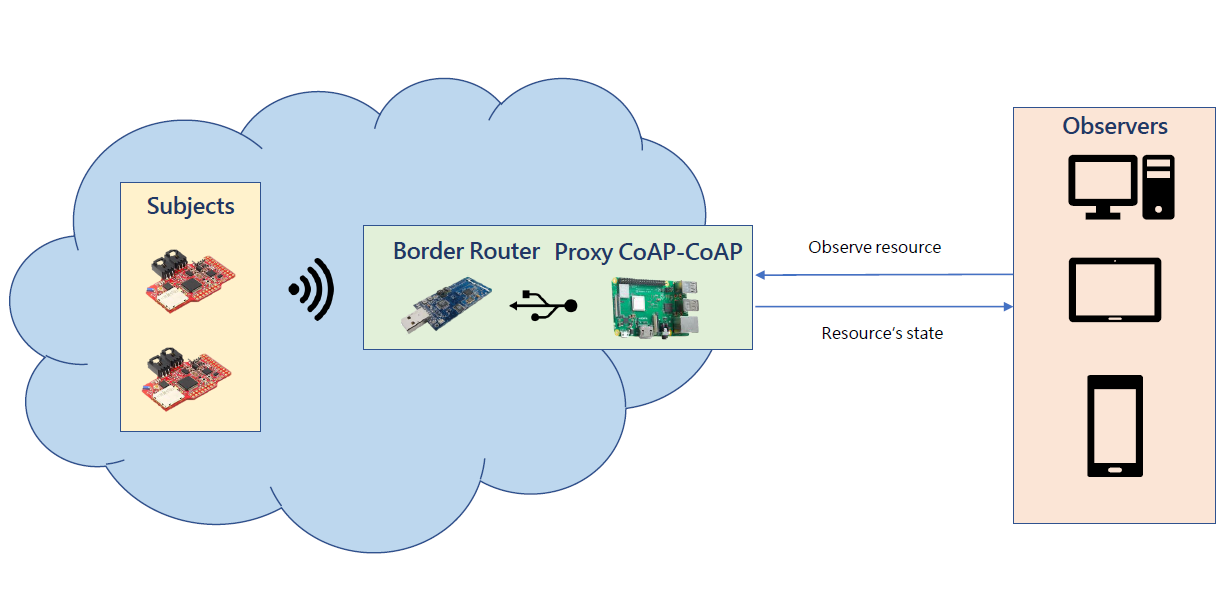
\includegraphics[width=\linewidth]{../Immagini/ArchitetturaGenerale.png}
    \caption{Ambiente di Testing}
    \label{fig:architettura}
  \end{figure}
  \section{Ritardo Trasmissione}
    Seguendo il meccanismo di tramissione spiegato in \ref{NotificaPriotita}, il \textit{ProxyObserver} invia le notifiche in modo ordinato agli osservatori, nel seguente ordine:
    \begin{enumerate}
      \item \textbf{CoAP.QoSLevel.CRITICAL\_HIGHEST\_PRIORITY}
      \item \textbf{CoAP.QoSLevel.CRITICAL\_HIGH\_PRIORITY}
      \item \textbf{CoAP.QoSLevel.NON\_CRITICAL\_MEDIUM\_PRIORITY}
      \item \textbf{CoAP.QoSLevel.NON\_CRITICAL\_LOW\_PRIORITY}
    \end{enumerate}
    Questo si riflette sul tempo necessario ad un osservatore a ricevere la propria notifica, in particolare gli osservatori registrati sulla stessa risorsa dello stesso sensore, riceveranno le notifiche in istanti diversi dipendentemente dal loro livello di priorità.
    Il testing effettuato permette di evidenziare questa conseguenza del nuovo meccanismo di invio e si basa sull'acquisizione del timestamp in 2 istanti precisi:
    \begin{enumerate}
      \item Istante di \textbf{invio} della notifica da parte del \textit{Subject}
      \item Istante di \textbf{ricezione} della notifica da parte del \textit{Observer}
    \end{enumerate}
    Sono stati avviati 16 Observer, in particolare 4 Observer per ogni priorità. Questi hanno richiesto al Proxy le notifiche della temperatura di un sensore, simulando che quest'ultimo sia costantemente in una situazione di criticità, in modo che tutti gli observer ricevino lo stesso numero di notifiche. \newline
    L'esecuzione è proseguita per un certo intervallo di tempo in cui sono state ricevute circa 40 notifiche, per ognuno delle quali sono stati salvati i timestamp di ricezione in un log relativo ad ogni observer, oltre al log del Subject in cui sono stati salvati i timestamp di invio. A questo punto, è stato possibile analizzare i file creati tramite uno script Python che calcola il ritardo di trasmissione medio dei pacchetti per ogni priorità. \newline
    I risultati ottenuti variano in base all'ambiente in cui sono stati effettuati i testing, in particolare:
    \begin{itemize}
      \item Canale di comunicazione con poche interferenze \ref{fig:graficoRitardoLibero}
      \item Canale di comunicazione abbastanza disturbato \ref{fig:graficoRitardoDisturbato}
    \end{itemize}
    In entrambi è evidente come all'aumentare della priorità il ritardo medio si riduce.
    \begin{figure}
      \centering
      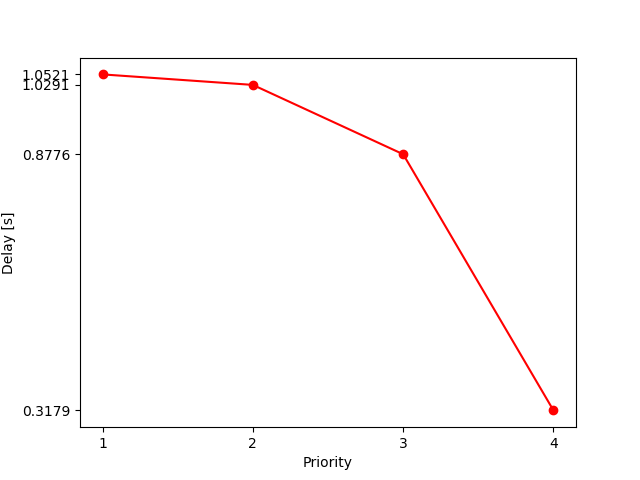
\includegraphics[scale = 0.75]{../Immagini/GraficoRitardoLibero.png}
      \caption{Grafico del ritardo al variare della priorità degli Observer con canale libero}
      \label{fig:graficoRitardoLibero}
    \end{figure}
    \begin{figure}
      \centering
      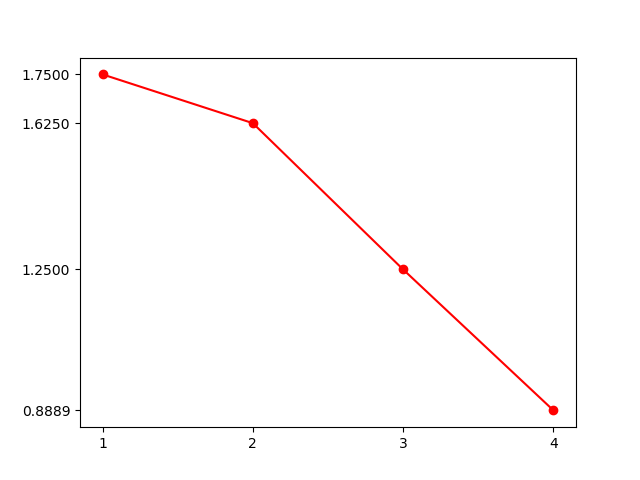
\includegraphics[scale = 0.75]{../Immagini/GraficoRitardoDisturbato.png}
      \caption{Grafico del ritardo al variare della priorità degli Observer con canale disturbato}
      \label{fig:graficoRitardoDisturbato}
    \end{figure}

    \section{Consumo Batteria in funzione del Numero di Pacchetti}

    saldgsaljydgsalydvasydgsaydg asldg sauldgsayd gsaduylgs ayludgasu lgaslu dygaslud gasludy gasljd gasljdg auldg alsugd aludgausdgaudgausl
    saldgsaljydgsalydvasydgsaydg asldg sauldgsayd gsaduylgs ayludgasu lgaslu dygaslud gasludy gasljd gasljdg auldg alsugd aludgausdgaudgausl
    saldgsaljydgsalydvasydgsaydg asldg sauldgsayd gsaduylgs ayludgasu lgaslu dygaslud gasludy gasljd gasljdg auldg alsugd aludgausdgaudgausl
    saldgsaljydgsalydvasydgsaydg asldg sauldgsayd gsaduylgs ayludgasu lgaslu dygaslud gasludy gasljd gasljdg auldg alsugd aludgausdgaudgausl
    saldgsaljydgsalydvasydgsaydg asldg sauldgsayd gsaduylgs ayludgasu lgaslu dygaslud gasludy gasljd gasljdg auldg alsugd aludgausdgaudgausl
    saldgsaljydgsalydvasydgsaydg asldg sauldgsayd gsaduylgs ayludgasu lgaslu dygaslud gasludy gasljd gasljdg auldg alsugd aludgausdgaudgausl
    saldgsaljydgsalydvasydgsaydg asldg sauldgsayd gsaduylgs ayludgasu lgaslu dygaslud gasludy gasljd gasljdg auldg alsugd aludgausdgaudgausl
    saldgsaljydgsalydvasydgsaydg asldg sauldgsayd gsaduylgs ayludgasu lgaslu dygaslud gasludy gasljd gasljdg auldg alsugd aludgausdgaudgausl
    saldgsaljydgsalydvasydgsaydg asldg sauldgsayd gsaduylgs ayludgasu lgaslu dygaslud gasludy gasljd gasljdg auldg alsugd aludgausdgaudgausl
      \begin{center}
        \begin{figure}
          \centering
          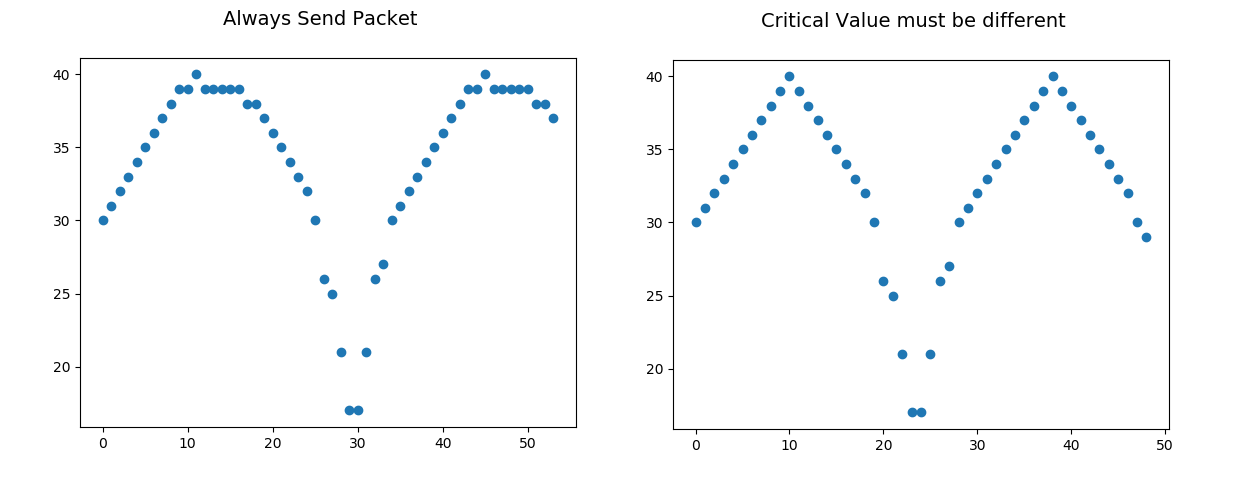
\includegraphics[width=\linewidth]{../Immagini/MergeOn.png}
          \caption{Grafici Pacchetti Inviati con Algoritmo attivo}
          \label{fig:mergeOn}
        \end{figure}

        \begin{figure}
          \centering
          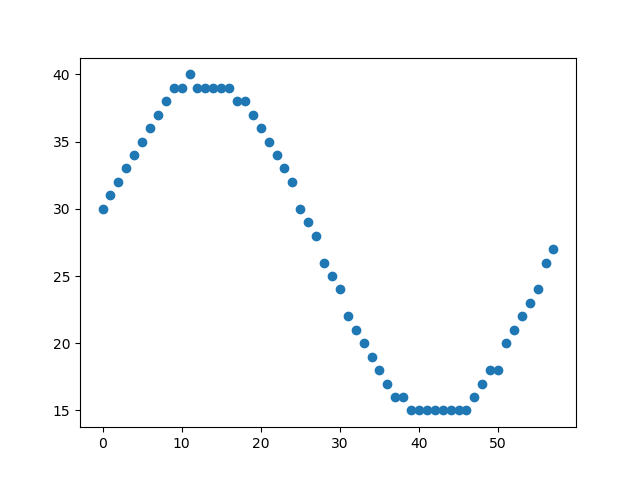
\includegraphics[width=\linewidth]{../Immagini/OFF.png}
          \caption{Grafici Pacchetti Inviati con Algoritmo disattivato}
          \label{fig:off}
        \end{figure}
      \end{center}

      saldgsaljydgsalydvasydgsaydg asldg sauldgsayd gsaduylgs ayludgasu lgaslu dygaslud gasludy gasljd gasljdg auldg alsugd aludgausdgaudgausl
      saldgsaljydgsalydvasydgsaydg asldg sauldgsayd gsaduylgs ayludgasu lgaslu dygaslud gasludy gasljd gasljdg auldg alsugd aludgausdgaudgausl
      saldgsaljydgsalydvasydgsaydg asldg sauldgsayd gsaduylgs ayludgasu lgaslu dygaslud gasludy gasljd gasljdg auldg alsugd aludgausdgaudgausl
      saldgsaljydgsalydvasydgsaydg asldg sauldgsayd gsaduylgs ayludgasu lgaslu dygaslud gasludy gasljd gasljdg auldg alsugd aludgausdgaudgausl
      saldgsaljydgsalydvasydgsaydg asldg sauldgsayd gsaduylgs ayludgasu lgaslu dygaslud gasludy gasljd gasljdg auldg alsugd aludgausdgaudgausl





    \section{Variazione MaxAge}
      L'algoritmo descritto nel capitolo delle Specifiche \ref{Spec:MaxAge} è stato realizzato apportando delle leggere modifiche ai parametri utilizzati per la modifica del valore del MaxAge. I parametri adottati sono riportarti in tabella \ref{tab:Parametri}

      \newcolumntype{P}[1]{>{\centering\arraybackslash}p{#1}}
        \begin{table}%[!h]
          \renewcommand{\arraystretch}{1.2}
           \caption{Parametri per la Variazione del MaxAge}
           \label{tab:Parametri}
           \centering
             \begin{tabular}{  P{7cm}  P{7cm}  }
                 \firsthline
                 \cline{1-2}
                 \textbf{Parametro} & \textbf{Valore} \\
               \hline
                  RESOURCES\_SENSING\_PERIOD & 5 \\
                  STEP & 2 \\
                  MAX\_AGE\_THRESHOLD & 10 \\
                  RESOURCE\_MIN\_MAX\_AGE & RESOURCES\_SENSING\_PERIOD + MAX\_AGE\_THRESHOLD \\
                  RESOURCE\_MAX\_AGE & 15*RESOURCES\_SENSING\_PERIOD + MAX\_AGE\_THRESHOLD \\
                \lasthline
             \end{tabular}
        \end{table}
      Il testing è stato eseguito simulando uno scenario in cui i valori rimangono per la maggior parte del tempo costanti, nel caso specifico ad una temperatura di \ang{28}, con dei picchi a \ang{33} per simulare l'arrivo di un valore critico. Nella figura \ref{fig:graficoMaxAge} si può notare come subito dopo l'arrivo di un valore critico, la frequenza di arrivo delle notifiche dimunisce nel tempo dato che il MaxAge aumenta. Questo accade in quanto per evitare che l'observer cancelli la relazione di osservazione in seguito alla scadenza del MaxAge, il subject invia una nuova notifica prima della scandena, nello specifico RESOURCES\_SENSING\_PERIOD secondi. I parametri utilizzati dovranno essere settati in base alla tipologia della risorsa.
      \begin{figure}
        \centering
        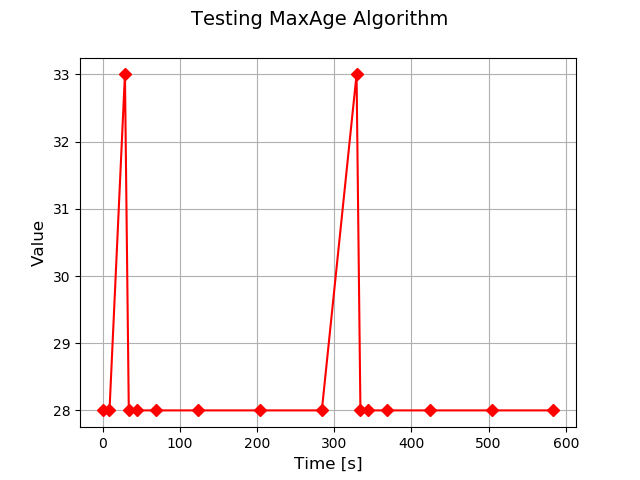
\includegraphics[scale=0.75]{../Immagini/MaxAge.png}
        \caption{Grafico della variazione del MaxAge quando il valore rimane costante}
        \label{fig:graficoMaxAge}
      \end{figure}
